

\section{Introduction}

The two-phase optimisation via simulation of healthcare Emergency
Departments, ED, proposed in \ref{ch3:Proposed-OvS-ED} was applied
herewith to analyse the administrative strategies leading to optimum
decisions about the physical and human resources of an ED. In particular,
the impact on the economics and the productivity of Sabadell Hospital
ED of different sanitary staff configuration (v.gr., doctors, triage
nurses, admission personnel, emergency nurses, and x-ray technicians)
were analysed. It is a discrete combinatorial optimisation problem.

There are three main issues to be addressed to carry out the evaluation,
namely: the \textit{simulation models} that represent the system under
study (discussed along the previous chapters); the \textit{decision
variables} and\textit{ workloads} used as inputs of the simulation
models; and the \textit{metrics} used to asses the benefits of the
proposal. We have defined some significant workloads and a set of
metrics to observe both functional and performance features of the
proposal. This set of metrics were defined in term of three different
indexes, namely: patient length of stay (LoS) in the ED; number of
attended patients per day (Throughput); and a compound index, the
product of the cost of a given sanitary staff configuration times
patient length of stay (CLoS).

In the following sections, the \textit{decision variables, }the\textit{
workloads}, and the \textit{metrics} are described. Finally two case
scenarios and their results are presented and discussed. 


\section{Field Information of Sabadell Hospital ED}

It was found through interviews with the managers at the EDs of Sabadell
hospital (which provides healthcare services to an average of 160,000
patients/year), it was found that a basic sanitary of its ED staff
is composed by: doctors, triage nurses, emergency nurses, admission
personnel, and x-ray technicians, as shown in \ref{tab:T1}. This
table also shows some characteristics of such sanitary staff, namely:
sort of staff as junior or senior (that represents less and more expertise,
respectively); their respective costs (� \textbf{}%
\footnote{\textbf{It is not an actual euro, could be any currency.\label{fn:euro}}%
}); the operational patient-service-time (hours); and the minimum and
maximum number of each kind of staff. 

\begin{comment}
 %
\saveFN\mymark  %
\end{comment}
\foreignlanguage{american}{}%
\begin{comment}
 %
\useFN\mymark  %
\end{comment}


\begin{table}[H]
\caption{Sabadell Hospital ED staff and their: associated expertise, costs,
operational patient-service time, and number.}


\begin{centering}
\begin{tabular}{>{\centering}m{3.5cm}>{\centering}p{1.1cm}>{\centering}p{1cm}>{\centering}p{1.1cm}>{\centering}p{1cm}>{\centering}m{0.075cm}>{\centering}m{2.2cm}}
\cline{1-5} \cline{7-7} 
\multicolumn{1}{>{\centering}m{3.5cm}|}{\textbf{Sanitary staff} } & \multicolumn{2}{c|}{\textbf{Cost (�$^{1}$)}} & \multicolumn{2}{c}{\textbf{Time/patient (hours)}} &  & \textbf{Number of personnel}\tabularnewline
\cline{1-5} \cline{7-7} 
 & Senior  & Junior  & Senior & Junior &  & min - Max\tabularnewline
\cline{1-5} \cline{7-7} 
Doctor  & 1000  & 500  & 0.26 & 0.35 &  & \textbf{\textit{1 -- 4}} \tabularnewline
\cline{1-5} \cline{7-7} 
Triage Nurse  & 500  & 350  & 0.09 & 0.13 &  & \textbf{\textit{1 -- 3}} \tabularnewline
\cline{1-5} \cline{7-7} 
Emergency Nurse & 500  & 350  & 0.14 & 0.18 &  & \textbf{\textit{1 -- 2}} \tabularnewline
\cline{1-5} \cline{7-7} 
Admission personnel & 200  & 150  & 0.02 & 0.035 &  & \textbf{\textit{1 -- 3}} \tabularnewline
\cline{1-5} \cline{7-7} 
X-ray technician & 200  & 150  & 0.09 & 0.14 &  & \textbf{\textit{1 -- 2}} \tabularnewline
\cline{1-5} \cline{7-7} 
\end{tabular}
\par\end{centering}

\label{tab:T1} 
\end{table}


\begin{figure}[H]
\centering 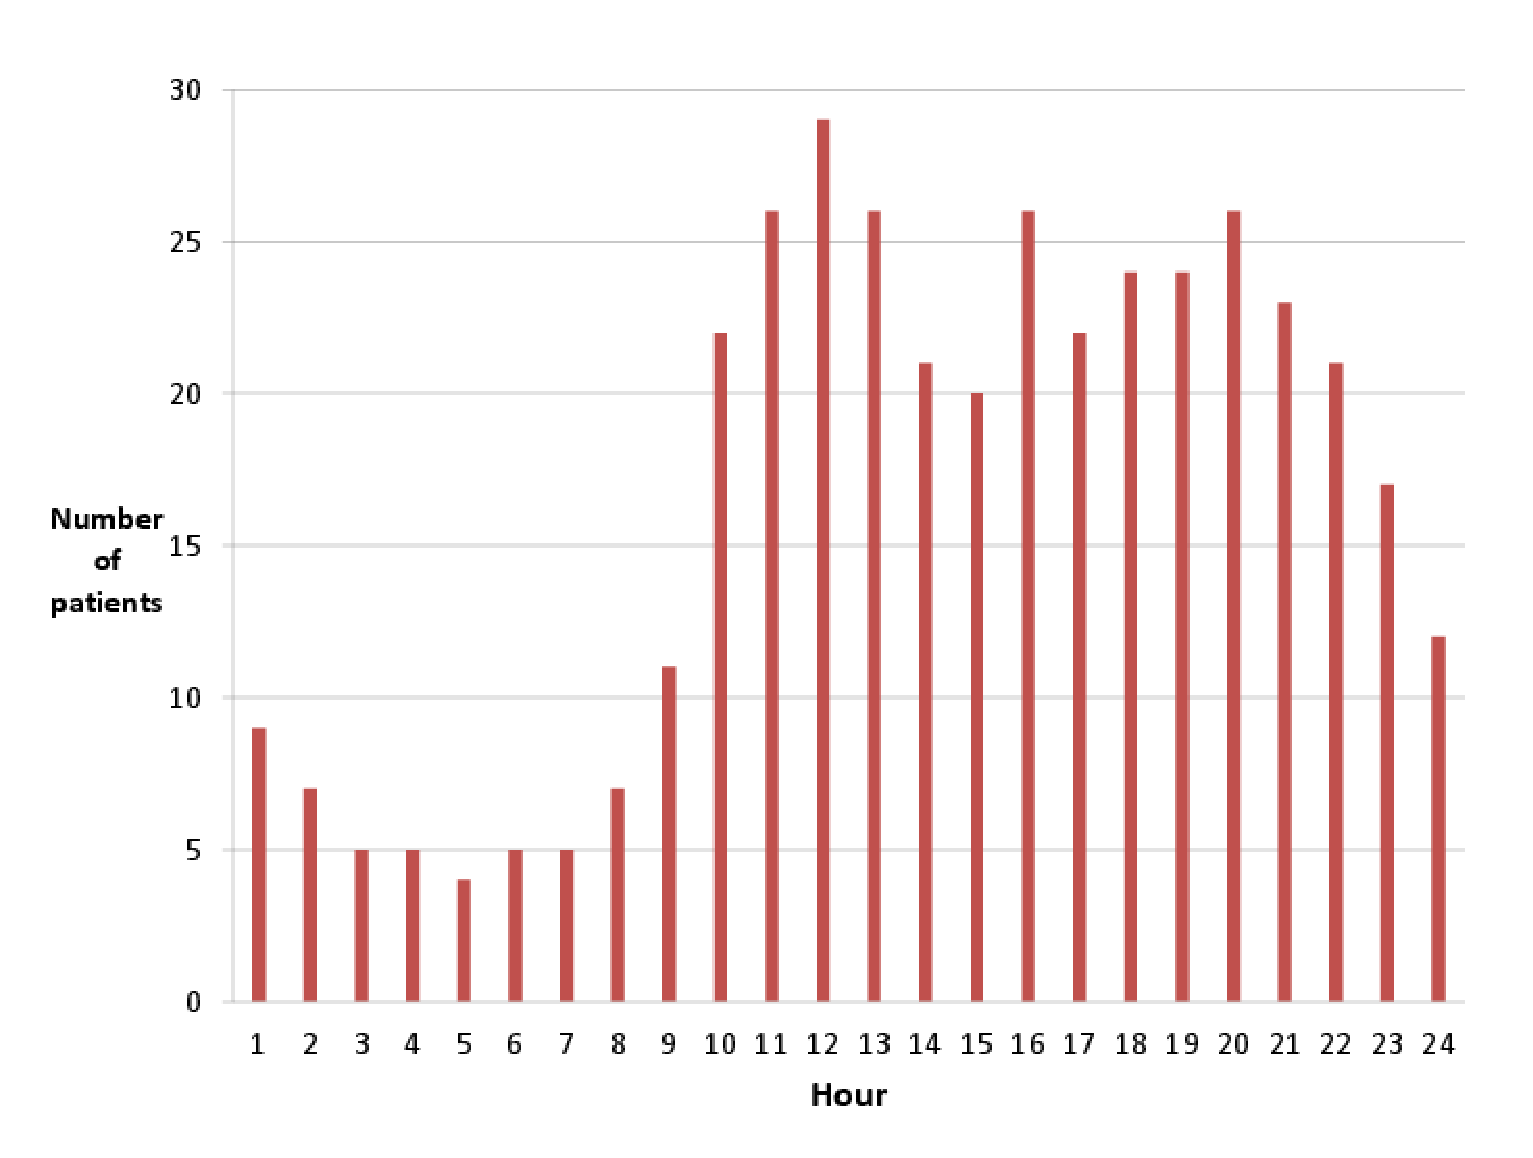
\includegraphics[width=0.85\columnwidth,height=0.17\paperheight]{figs4/input} 

\caption{Sabadell Hospital ED average of 400 daily incoming patients and its
hourly distribution (February 2010).\label{fig:real-input}}
\end{figure}


In reference to the Sabadell Hospital ED incoming patients, an average
of four hundred of patients daily arrive to the ED of Sabadell hospital.
As example, the statistics corresponding to February 2010, of this
real average number of incoming patients and its hourly distribution
are shown in \ref{fig:real-input}. As stated in \ref{sec:active-agents}
all incomings patients are triaged to identify the acuity of them
and to prioritise their urgency of attention. Thus, the average percentage,
according to the priority level of urgency of attention, of the incoming
patients to the ED of Sabadell hospital is as follows: triage level
1 - 1\%; triage level 2 - 4\%; triage level 3 - 20\%; triage level
4 - 32\%;and triage level 5 - 43\%. Patients identified as triage
level 4 and triage level 5 represent up to 75\% of the total of the
incoming patients to the ED of Sabadell hospital.

\begin{comment}
All simulations were done using the simulator previously explained,
utilising the \emph{BehaviorSpace} tool, serially and using the cluster
\textit{IBM} of the department, which has 32 Compute nodes with 2
x Dual-Core Intel(R) Xeon(R) CPU 5160 running at 3.00GHz, with 12
GB of RAM, and 4MB of L2 share cache (2x2)
\end{comment}


%\begin{figure}[htb!] 
%\centering 
%\begin{tabular}{ccc} 	
%	\subfloat[][9 Admission (A) personnel staff cases. AD\textit{i} represents Admission Den %\textit{i}.] 
%{\label{subfloat:adm_comb} 
%\resizebox{1.7in}{!} { 
%\begin{tabular}{cccc} 
%\hline 
%Case number & \bf{AD$_1$} & \bf {AD$_2$}  & \bf {AD$_3$}  \\ \hline 
%1 & AS  & -  & -    \\ \hline 
%2 & AJ  & -  & -    \\ \hline 
%3 & AS  & AS  & -    \\ \hline 
%4 & AJ  & AJ  & -    \\ \hline 
%5 & AS  & AJ  & -    \\ \hline 
%6 & AS  & AS  & AS    \\ \hline 
%7 & AJ  & AJ  & AJ    \\ \hline 
%8 & AS  & AJ  & AJ    \\ \hline 
%9 & AS  & AS  & AJ    \\ \hline 
%\end{tabular} 
%}         
%} 
%& 	
%	\subfloat[][9 Nurse (N) cases. TR\textit{i} represents Triage Room \textit{i}.] 
%{\label{subfloat:nur_comb} 
%\resizebox{1.7in}{!} { 
%\begin{tabular}{cccc} 
%\hline 
%Case number & \bf {TR$_1$} & \bf {TR$_2$}  & \bf {TR$_3$}  \\ \hline 
%1 & NS  & -  & -    \\ \hline 
%2 & NJ  & -  & -    \\ \hline 
%3 & NS  & NS  & -   \\ \hline 
%4 & NJ  & NJ  & -   \\ \hline 
%5 & NS  & NJ  & -   \\ \hline 
%6 & NS  & NS  & NS  \\ \hline 
%7 & NJ  & NJ  & NJ  \\ \hline 
%8 & NS  & NJ  & NJ  \\ \hline 
%9 & NS  & NS  & NJ  \\ \hline 
%\end{tabular} 
%}         
%} 
%&         
%	\subfloat[][14 Doctor (D) cases.  DR\textit{i} represents Diagnosis Room \textit{i}.] 
%{\label{subfloat:doc_comb} 
%\resizebox{1.99in}{!} {
%\begin{tabular}{ccccc} 
%\hline 
%Case number & \bf {DR$_1$} & \bf {DR$_2$}  & \bf {DR$_3$}  & \bf {DR$_4$}  \\ \hline 
%1 & DS  & -  & -  & -  \\ \hline 
%2 & DJ  & -  & -  & -  \\ \hline 
%3 & DS  & DS  & -  & -  \\ \hline 
%4 & DJ  & DJ  & -  & -  \\ \hline 
%5 & DS  & DJ  & -  & -  \\ \hline 
%6 & DS  & DS  & DS  & -  \\ \hline 
%7 & DJ  & DJ  & DJ  & -  \\ \hline 
%8 & DS  & DJ  & DJ  & -  \\ \hline 
%9 & DS  & DS  & DJ  & -  \\ \hline 
%10 & DS  & DS  & DS  & DS  \\ \hline 
%11 & DJ  & DJ  & DJ  & DJ  \\ \hline 
%12 & DS  & DJ  & DJ  & DJ  \\ \hline 
%13 & DS  & DS  & DJ  & DJ  \\ \hline 
%14 & DS  & DS  & DS  & DJ  \\ \hline 
%\end{tabular} 
%}       
% } 
%\end{tabular} 
%\caption{Combinations of sanitary staff: Admission (A) personnel, Nurses (N) and Doctors (D). Two levels of expertise: Junior (J), and Senior (S).} 
%\label{fig:combs} 
%\end{figure} 



\section{Decision Variables of Sabadell Hospital ED}

The sanitary staff included in \ref{tab:T1} are the \textit{decision
variables} of the ED. 
\begin{table}[H]
\noindent \begin{centering}
\hfill{}%
\begin{minipage}[t]{0.45\columnwidth}%
\centering\resizebox{2.3in}{!}{%%
\begin{tabular}{>{\centering}m{1.4cm}>{\centering}m{1.2cm}>{\centering}m{1.2cm}>{\centering}m{1.2cm}}
\hline 
Case number & \textbf{AD\textsubscript{1} } & \textbf{AD\textsubscript{2}} & \textbf{AD\textsubscript{3}}\tabularnewline
\hline 
1 & AS & - & -\tabularnewline
2 & AJ & - & -\tabularnewline
3 & AS & AS & -\tabularnewline
4 & AJ & AJ & -\tabularnewline
5 & AS & AJ & -\tabularnewline
6 & AS & AS & AS\tabularnewline
7 & AJ & AJ & AJ\tabularnewline
8 & AS & AJ & AJ\tabularnewline
9 & AS & AS & AJ\tabularnewline
\hline 
\end{tabular}}

\caption{9 Admission (A) personnel cases. AD\textit{\textsubscript{\textit{i}}}
is Admission Den\textit{\textsubscript{\textit{i}}}.$\,$Where AJ
means Admission personnel Junior, whereas AS means Admission personnel
Senior. \label{subtab:As}}
%
\end{minipage}\hfill{}%
\begin{minipage}[t]{0.45\columnwidth}%
\centering\resizebox{2.3in}{!}{%%
\begin{tabular}{>{\centering}m{1.4cm}>{\centering}m{1.2cm}>{\centering}m{1.2cm}>{\centering}m{1.2cm}}
\hline 
Case number & \textbf{TR\textsubscript{1}} & \textbf{TR\textsubscript{2}} & \textbf{TR\textsubscript{3}}\tabularnewline
\hline 
1 & NS & - & -\tabularnewline
2 & NJ & - & -\tabularnewline
3 & NS & NS & -\tabularnewline
4 & NJ & NJ & -\tabularnewline
5 & NS & NJ & -\tabularnewline
6 & NS & NS & NS\tabularnewline
7 & NJ & NJ & NJ\tabularnewline
8 & NS & NJ & NJ\tabularnewline
9 & NS & NS & NJ\tabularnewline
\hline 
\end{tabular}}

\caption{9 Nurse (N) cases. TR\textit{\textsubscript{\textit{i}}} represents
Triage Room \emph{i}. Where NJ means Triage Nurse Junior, whereas
NS means Triage Nurse Senior.\foreignlanguage{american}{\label{subtab:Ns}}}
%
\end{minipage}\hfill{}\vspace{0.1cm}

\par\end{centering}

\noindent \centering{}\hfill{}%
\begin{minipage}[t]{0.45\columnwidth}%
\centering\resizebox{1.7in}{!}{%
\begin{tabular}{>{\centering}m{1.4cm}>{\centering}m{1.4cm}>{\centering}m{1.4cm}}
\hline 
Case number & \textbf{ENR\textsubscript{1} } & \textbf{ENR\textsubscript{2}}\tabularnewline
\hline 
1 & ENS & -\tabularnewline
2 & ENJ & -\tabularnewline
3 & ENS & ENS\tabularnewline
4 & ENJ & ENJ\tabularnewline
5 & ENS & ENJ\tabularnewline
\hline 
\end{tabular}}

\caption{5 Emergency nurse (EN) cases. EN\textit{R\textsubscript{\textit{i}}}
represents ENurse Room \emph{i}. Where ENJ means Emergency Nurse Junior,
whereas ENS means Emergency Nurse Senior\foreignlanguage{american}{\label{subtab:ENs}}}
%
\end{minipage}\hfill{}%
\begin{minipage}[t]{0.45\columnwidth}%
\centering\resizebox{1.7in}{!}{%%
\begin{tabular}{>{\centering}m{1.4cm}>{\centering}m{1.4cm}>{\centering}m{1.4cm}}
\hline 
Case number & \textbf{XR\textsubscript{1}} & \textbf{XR\textsubscript{2}}\tabularnewline
\hline 
1 & XRS & -\tabularnewline
2 & XRJ & -\tabularnewline
3 & XRS & XRS\tabularnewline
4 & XRJ & XRJ\tabularnewline
5 & XRS & XRJ\tabularnewline
\hline 
\end{tabular}}

\caption{5 X-ray technician (XR) cases. XR\textit{\textsubscript{\textit{i}}}
represents X-ray Room \emph{i}. Where XRJ means X-ray technician Junior,
whereas XRS means X-ray technician Senior\foreignlanguage{american}{\label{subtab:Xrs}}}
%
\end{minipage}\hfill{}
\end{table}
 The disaggregation of \ref{tab:T1} yields \ref{subtab:As}, which
includes 9 possible combinations of admission personnel (junior/senior);
\ref{subtab:Ns}, which also includes 9 possible combinations of triage
nurses (junior/senior); \ref{subtab:ENs}, that presents the 5 possible
combinations of emergency nurse (junior/senior); \ref{subtab:Xrs}
that shows the 5 possible combinations of x-ray technician (junior/senior);
and \ref{subtab:Ds}, with 14 possible combinations of doctors (junior/senior)
in which the examined cases for each type of staff were included.
It is a discrete combinatorial problem.

 %
\begin{table}[H]
\caption{  %
14 Doctor (D) cases. DR\textit{\textsubscript{\textit{i}}} represents
Diagnosis Room \emph{i}. Where DJ means Doctor Junior, whereas DS
means Doctor Senior\foreignlanguage{american}{.\label{subtab:Ds}} %
}
\centering\resizebox{2.6in}{!}{%%
\begin{tabular}{>{\centering}m{1.4cm}>{\centering}m{1.1cm}>{\centering}m{1.1cm}>{\centering}m{1.1cm}>{\centering}m{1.1cm}}
\hline 
  %
Case number %
 &   %
\textbf{DR\textsubscript{1}} %
 &   %
\textbf{DR\textsubscript{2} } %
 &   %
\textbf{DR\textsubscript{3}} %
 &   %
\textbf{DR\textsubscript{4}} %
\tabularnewline
\hline 
  %
1 %
 &   %
DS %
 &   %
- %
 &   %
- %
 &   %
- %
\tabularnewline
  %
2 %
 &   %
DJ %
 &   %
- %
 &   %
- %
 &   %
- %
\tabularnewline
  %
3 %
 &   %
DS %
 &   %
DS %
 &   %
- %
 &   %
- %
\tabularnewline
  %
4 %
 &   %
DJ %
 &   %
DJ %
 &   %
- %
 &   %
- %
\tabularnewline
  %
5 %
 &   %
DS %
 &   %
DJ %
 &   %
- %
 &   %
- %
\tabularnewline
  %
6 %
 &   %
DS %
 &   %
DS %
 &   %
DS %
 &   %
- %
\tabularnewline
  %
7 %
 &   %
DJ %
 &   %
DJ %
 &   %
DJ %
 &   %
- %
\tabularnewline
  %
8 %
 &   %
DS %
 &   %
DJ %
 &   %
DJ %
 &   %
- %
\tabularnewline
  %
9 %
 &   %
DS %
 &   %
DS %
 &   %
DJ %
 &   %
- %
\tabularnewline
  %
10 %
 &   %
DS %
 &   %
DS %
 &   %
DS %
 &   %
DS %
\tabularnewline
  %
11 %
 &   %
DJ %
 &   %
DJ %
 &   %
DJ %
 &   %
DJ %
\tabularnewline
  %
12 %
 &   %
DS %
 &   %
DJ %
 &   %
DJ %
 &   %
DJ %
\tabularnewline
  %
13 %
 &   %
DS %
 &   %
DS %
 &   %
DJ %
 &   %
DJ %
\tabularnewline
  %
14 %
 &   %
DS %
 &   %
DS %
 &   %
DS %
 &   %
DJ %
\tabularnewline
\hline 
\end{tabular}}
\end{table}


  %
\ref{subtab:As} to \ref{subtab:Ds} were ordered by the sort and
number of staff, whereas \ref{subtab:As-pipe} to \ref{subtab:XRs-pipe}
were ordered by the equivalent operational patient-service time \foreignlanguage{american}{(t{*})}
of a ``single one'' sanitary professional (working in parallel)
of each sanitary staff configuration (admission personnel, nurses,
doctors, and x-ray technicians). This order was obtained by applying
the pipeline scheme described in \ref{sub:Pipeline-Model-ED} and
is graphically shown in \ref{fig:3D-scattered-LoS-wo} to \ref{fig:3D-scattered-LoS-tpipe}.
In these figures the index value was represented by colours, the most
important values in such figures were the green ones. 
\begin{table}[h]
 %
\caption{  %
Ordering staff configuration of admission personnel according to the
equivalent operational patient-service time \foreignlanguage{american}{(t{*})}
of each staff configuration.\label{subtab:As-pipe} %
}
\centering\resizebox{4.5in}{!}{%%
\begin{tabular}{>{\centering}m{1.4cm}>{\centering}m{1.4cm}>{\centering}m{1.2cm}>{\centering}m{1.2cm}>{\centering}m{1.2cm}>{\centering}m{1.2cm}>{\centering}m{1.2cm}>{\centering}m{1.2cm}}
\hline 
  %
Case number (t{*}) %
 &   %
Old case number %
 &   %
\textbf{AD\textsubscript{1} } %
 &   %
\textbf{AD\textsubscript{2}} %
 &   %
\textbf{AD\textsubscript{3}} %
 &   %
\textbf{�} %
 &   %
\textbf{Time (hrs)} %
 &   %
\textbf{t{*}}

\textbf{(hrs)} %
\tabularnewline
\hline 
  %
1 %
 &   %
6 %
 &   %
AS %
 &   %
AS %
 &   %
AS %
 &   %
600 %
 &   %
0.02 %
 &   %
0.007 %
\tabularnewline
  %
2 %
 &   %
9 %
 &   %
AS %
 &   %
AS %
 &   %
AJ %
 &   %
550 %
 &   %
0.035 %
 &   %
0.008 %
\tabularnewline
  %
3 %
 &   %
8 %
 &   %
AS %
 &   %
AJ %
 &   %
AJ %
 &   %
500 %
 &   %
0.035 %
 &   %
0.009 %
\tabularnewline
  %
4 %
 &   %
3 %
 &   %
AS %
 &   %
AS %
 &   %
- %
 &   %
400 %
 &   %
0.02 %
 &   %
0.001 %
\tabularnewline
  %
5 %
 &   %
7 %
 &   %
AJ %
 &   %
AJ %
 &   %
AJ %
 &   %
450 %
 &   %
0.035 %
 &   %
0.012 %
\tabularnewline
  %
6 %
 &   %
5 %
 &   %
AS %
 &   %
AJ %
 &   %
- %
 &   %
350 %
 &   %
0.035 %
 &   %
0.013 %
\tabularnewline
  %
7 %
 &   %
4 %
 &   %
AJ %
 &   %
AJ %
 &   %
- %
 &   %
300 %
 &   %
0.035 %
 &   %
0.018 %
\tabularnewline
  %
8 %
 &   %
1 %
 &   %
AS %
 &   %
- %
 &   %
- %
 &   %
200 %
 &   %
0.02 %
 &   %
0.02 %
\tabularnewline
  %
9 %
 &   %
2 %
 &   %
AJ %
 &   %
- %
 &   %
- %
 &   %
150 %
 &   %
0.035 %
 &   %
0.035 %
\tabularnewline
\hline 
\end{tabular}}  %
\end{table}
 
\begin{table}[h]
 %
\caption{  %
Ordering staff configuration of triage nurses according to the equivalent
operational patient-service time \foreignlanguage{american}{(t{*})}
of each staff configuration.\label{subtab:Ns-pipe} %
}
\centering\resizebox{4.5in}{!}{%%
\begin{tabular}{>{\centering}m{1.4cm}>{\centering}m{1.4cm}>{\centering}m{1.2cm}>{\centering}m{1.2cm}>{\centering}m{1.2cm}>{\centering}m{1.2cm}>{\centering}m{1.2cm}>{\centering}m{1.2cm}}
\hline 
  %
Case number (t{*}) %
 &   %
Old case number %
 &   %
\textbf{TR\textsubscript{1} } %
 &   %
\textbf{TR\textsubscript{2}} %
 &   %
\textbf{TR\textsubscript{3}} %
 &   %
\textbf{�} %
 &   %
\textbf{Time (hrs)} %
 &   %
\textbf{t{*}}

\textbf{(hrs)} %
\tabularnewline
\hline 
  %
1 %
 &   %
6 %
 &   %
NS %
 &   %
NS %
 &   %
NS %
 &   %
1,500 %
 &   %
0.09 %
 &   %
0.03 %
\tabularnewline
  %
2 %
 &   %
9 %
 &   %
NS %
 &   %
NS %
 &   %
NJ %
 &   %
1,350 %
 &   %
0.13 %
 &   %
0.033 %
\tabularnewline
  %
3 %
 &   %
8 %
 &   %
NS %
 &   %
NJ %
 &   %
NJ %
 &   %
1,200 %
 &   %
0.13 %
 &   %
0.04 %
\tabularnewline
  %
4 %
 &   %
7 %
 &   %
NJ %
 &   %
NJ %
 &   %
NJ %
 &   %
1,050 %
 &   %
0.13 %
 &   %
0.043 %
\tabularnewline
  %
5 %
 &   %
3 %
 &   %
NS %
 &   %
NS %
 &   %
- %
 &   %
1,000 %
 &   %
0.09 %
 &   %
0.05 %
\tabularnewline
  %
6 %
 &   %
5 %
 &   %
NS %
 &   %
NJ %
 &   %
- %
 &   %
850 %
 &   %
0.13 %
 &   %
0.053 %
\tabularnewline
  %
7 %
 &   %
4 %
 &   %
NJ %
 &   %
NJ %
 &   %
- %
 &   %
700 %
 &   %
0.13 %
 &   %
0.07 %
\tabularnewline
  %
8 %
 &   %
1 %
 &   %
NS %
 &   %
- %
 &   %
- %
 &   %
500 %
 &   %
0.09 %
 &   %
0.09 %
\tabularnewline
  %
9 %
 &   %
2 %
 &   %
NJ %
 &   %
- %
 &   %
- %
 &   %
350 %
 &   %
0.13 %
 &   %
0.13 %
\tabularnewline
\hline 
\end{tabular}}  %
\end{table}
 \foreignlanguage{american}{}
\begin{table}[H]
 %
\caption{  %
Ordering staff configuration of doctors according to the equivalent
operational patient-service time \foreignlanguage{american}{(t{*})}
of each staff configuration.\foreignlanguage{american}{\label{subtab:Ds-pipe}} %
}
\centering\resizebox{4.8in}{!}{%%
\begin{tabular}{>{\centering}m{1.4cm}>{\centering}m{1.4cm}>{\centering}m{1.1cm}>{\centering}m{1.1cm}>{\centering}m{1.1cm}>{\centering}m{1.1cm}>{\centering}m{1.1cm}>{\centering}m{1.1cm}>{\centering}m{1.5cm}}
\hline 
  %
Case number (t{*}) %
 &   %
Old case number %
 &   %
\textbf{DR\textsubscript{1}} %
 &   %
\textbf{DR\textsubscript{2}} %
 &   %
\textbf{DR\textsubscript{3}} %
 &   %
\textbf{DR\textsubscript{4}} %
 &   %
\textbf{�} %
 &   %
\textbf{Time (hrs)} %
 &   %
\textbf{t{*}}

\textbf{(hrs)} %
\tabularnewline
\hline 
  %
1 %
 &   %
10 %
 &   %
DS %
 &   %
DS %
 &   %
DS %
 &   %
DS %
 &   %
4,000 %
 &   %
0.26 %
 &   %
0.065 %
\tabularnewline
  %
2 %
 &   %
14 %
 &   %
DS %
 &   %
DS %
 &   %
DS %
 &   %
DJ %
 &   %
3,500 %
 &   %
0.35 %
 &   %
0.069 %
\tabularnewline
  %
3 %
 &   %
13 %
 &   %
DS %
 &   %
DS %
 &   %
DJ %
 &   %
DJ %
 &   %
3,000 %
 &   %
0.35 %
 &   %
0.075 %
\tabularnewline
  %
4 %
 &   %
12 %
 &   %
DS %
 &   %
DJ %
 &   %
DJ %
 &   %
DJ %
 &   %
2,500 %
 &   %
0.35 %
 &   %
0.081 %
\tabularnewline
  %
5 %
 &   %
6 %
 &   %
DS %
 &   %
DS %
 &   %
DS %
 &   %
- %
 &   %
3,000 %
 &   %
0.26 %
 &   %
0.087 %
\tabularnewline
  %
6 %
 &   %
11 %
 &   %
DJ %
 &   %
DJ %
 &   %
DJ %
 &   %
DJ %
 &   %
2,000 %
 &   %
0.35 %
 &   %
0.09 %
\tabularnewline
  %
7 %
 &   %
9 %
 &   %
DS %
 &   %
DS %
 &   %
DJ %
 &   %
- %
 &   %
2,500 %
 &   %
0.35 %
 &   %
0.095 %
\tabularnewline
  %
8 %
 &   %
8 %
 &   %
DS %
 &   %
DJ %
 &   %
DJ %
 &   %
- %
 &   %
2,000 %
 &   %
0.35 %
 &   %
0.11 %
\tabularnewline
  %
9 %
 &   %
7 %
 &   %
DJ %
 &   %
DJ %
 &   %
DJ %
 &   %
- %
 &   %
1,500 %
 &   %
0.35 %
 &   %
0.117 %
\tabularnewline
  %
10 %
 &   %
3 %
 &   %
DS %
 &   %
DS %
 &   %
- %
 &   %
- %
 &   %
2,000 %
 &   %
0.26 %
 &   %
0.13 %
\tabularnewline
  %
11 %
 &   %
5 %
 &   %
DS %
 &   %
DJ %
 &   %
- %
 &   %
- %
 &   %
1,500 %
 &   %
0.35 %
 &   %
0.149 %
\tabularnewline
  %
12 %
 &   %
4 %
 &   %
DJ %
 &   %
DJ %
 &   %
- %
 &   %
- %
 &   %
1,000 %
 &   %
0.35 %
 &   %
0.175 %
\tabularnewline
  %
13 %
 &   %
1 %
 &   %
DS %
 &   %
- %
 &   %
- %
 &   %
- %
 &   %
1,000 %
 &   %
0.26 %
 &   %
0.26 %
\tabularnewline
  %
14 %
 &   %
2 %
 &   %
DJ %
 &   %
- %
 &   %
- %
 &   %
- %
 &   %
500 %
 &   %
0.35 %
 &   %
0.35 %
\tabularnewline
\hline 
\end{tabular}}  %
\end{table}


\begin{table}[H]
 %
\caption{  %
Ordering staff configuration of emergency nurses according to the
equivalent operational patient-service time \foreignlanguage{american}{(t{*})}
of each staff configuration. \label{subtab:ENs-pipe} %
}
\centering\resizebox{3.8in}{!}{%%
\begin{tabular}{>{\centering}m{1.4cm}>{\centering}m{1.4cm}>{\centering}m{1.4cm}>{\centering}m{1.4cm}>{\centering}m{1.2cm}>{\centering}m{1.2cm}>{\centering}m{1.2cm}}
\hline 
  %
Case number (t{*}) %
 &   %
Old case number %
 &   %
\textbf{ENR\textsubscript{1}} %
 &   %
\textbf{ENR\textsubscript{2}} %
 &   %
\textbf{�} %
 &   %
\textbf{Time (hrs)} %
 &   %
\textbf{t{*}}

\textbf{(hrs)} %
\tabularnewline
\hline 
  %
1 %
 &   %
3 %
 &   %
ENS %
 &   %
ENS %
 &   %
1,000 %
 &   %
0.14 %
 &   %
0.07 %
\tabularnewline
  %
2 %
 &   %
5 %
 &   %
ENS %
 &   %
ENJ %
 &   %
850 %
 &   %
0.18 %
 &   %
0.08 %
\tabularnewline
  %
3 %
 &   %
4 %
 &   %
ENJ %
 &   %
ENJ %
 &   %
700 %
 &   %
0.18 %
 &   %
0.09 %
\tabularnewline
  %
4 %
 &   %
1 %
 &   %
ENS %
 &   %
- %
 &   %
500 %
 &   %
0.14 %
 &   %
0.14 %
\tabularnewline
  %
5 %
 &   %
2 %
 &   %
ENJ %
 &   %
- %
 &   %
350 %
 &   %
0.18 %
 &   %
0.18 %
\tabularnewline
\hline 
\end{tabular}}  %
\end{table}
 
\begin{table}[H]
 %
\caption{  %
Ordering staff configuration of x-ray technicians according to the
equivalent operational patient-service time \foreignlanguage{american}{(t{*})}
of each staff configuration.\label{subtab:XRs-pipe} %
}
\centering\resizebox{3.8in}{!}{%%
\begin{tabular}{>{\centering}m{1.4cm}>{\centering}m{1.4cm}>{\centering}m{1.2cm}>{\centering}m{1.2cm}>{\centering}m{1.2cm}>{\centering}m{1.2cm}>{\centering}m{1.2cm}}
\hline 
  %
Case number (t{*}) %
 &   %
Old case number %
 &   %
\textbf{XR\textsubscript{1} } %
 &   %
\textbf{XR\textsubscript{2}} %
 &   %
\textbf{�} %
 &   %
\textbf{Time (hrs)} %
 &   %
\textbf{t{*}}

\textbf{(hrs)} %
\tabularnewline
\hline 
  %
1 %
 &   %
3 %
 &   %
XRS %
 &   %
XRS %
 &   %
400 %
 &   %
0.09 %
 &   %
0.045 %
\tabularnewline
  %
2 %
 &   %
5 %
 &   %
XRS %
 &   %
XRJ %
 &   %
350 %
 &   %
0.14 %
 &   %
0.055 %
\tabularnewline
  %
3 %
 &   %
4 %
 &   %
XRJ %
 &   %
XRJ %
 &   %
300 %
 &   %
0.14 %
 &   %
0.07 %
\tabularnewline
  %
4 %
 &   %
1 %
 &   %
XRS %
 &   %
- %
 &   %
200 %
 &   %
0.09 %
 &   %
0.09 %
\tabularnewline
  %
5 %
 &   %
2 %
 &   %
XRJ %
 &   %
- %
 &   %
150 %
 &   %
0.14 %
 &   %
0.14 %
\tabularnewline
\hline 
\end{tabular}}  %
\end{table}
 In the first example, \ref{fig:3D-scattered-LoS-wo} shows a 3D scattered
graph, which axes were ordered by the sort and number of sanitary
staff (first column/case number of \ref{subtab:As} to \ref{subtab:Ds}.
In this graph the green points were all scattered, and they shown
lack of connectivity. 
\begin{figure}[H]
\noindent \centering{}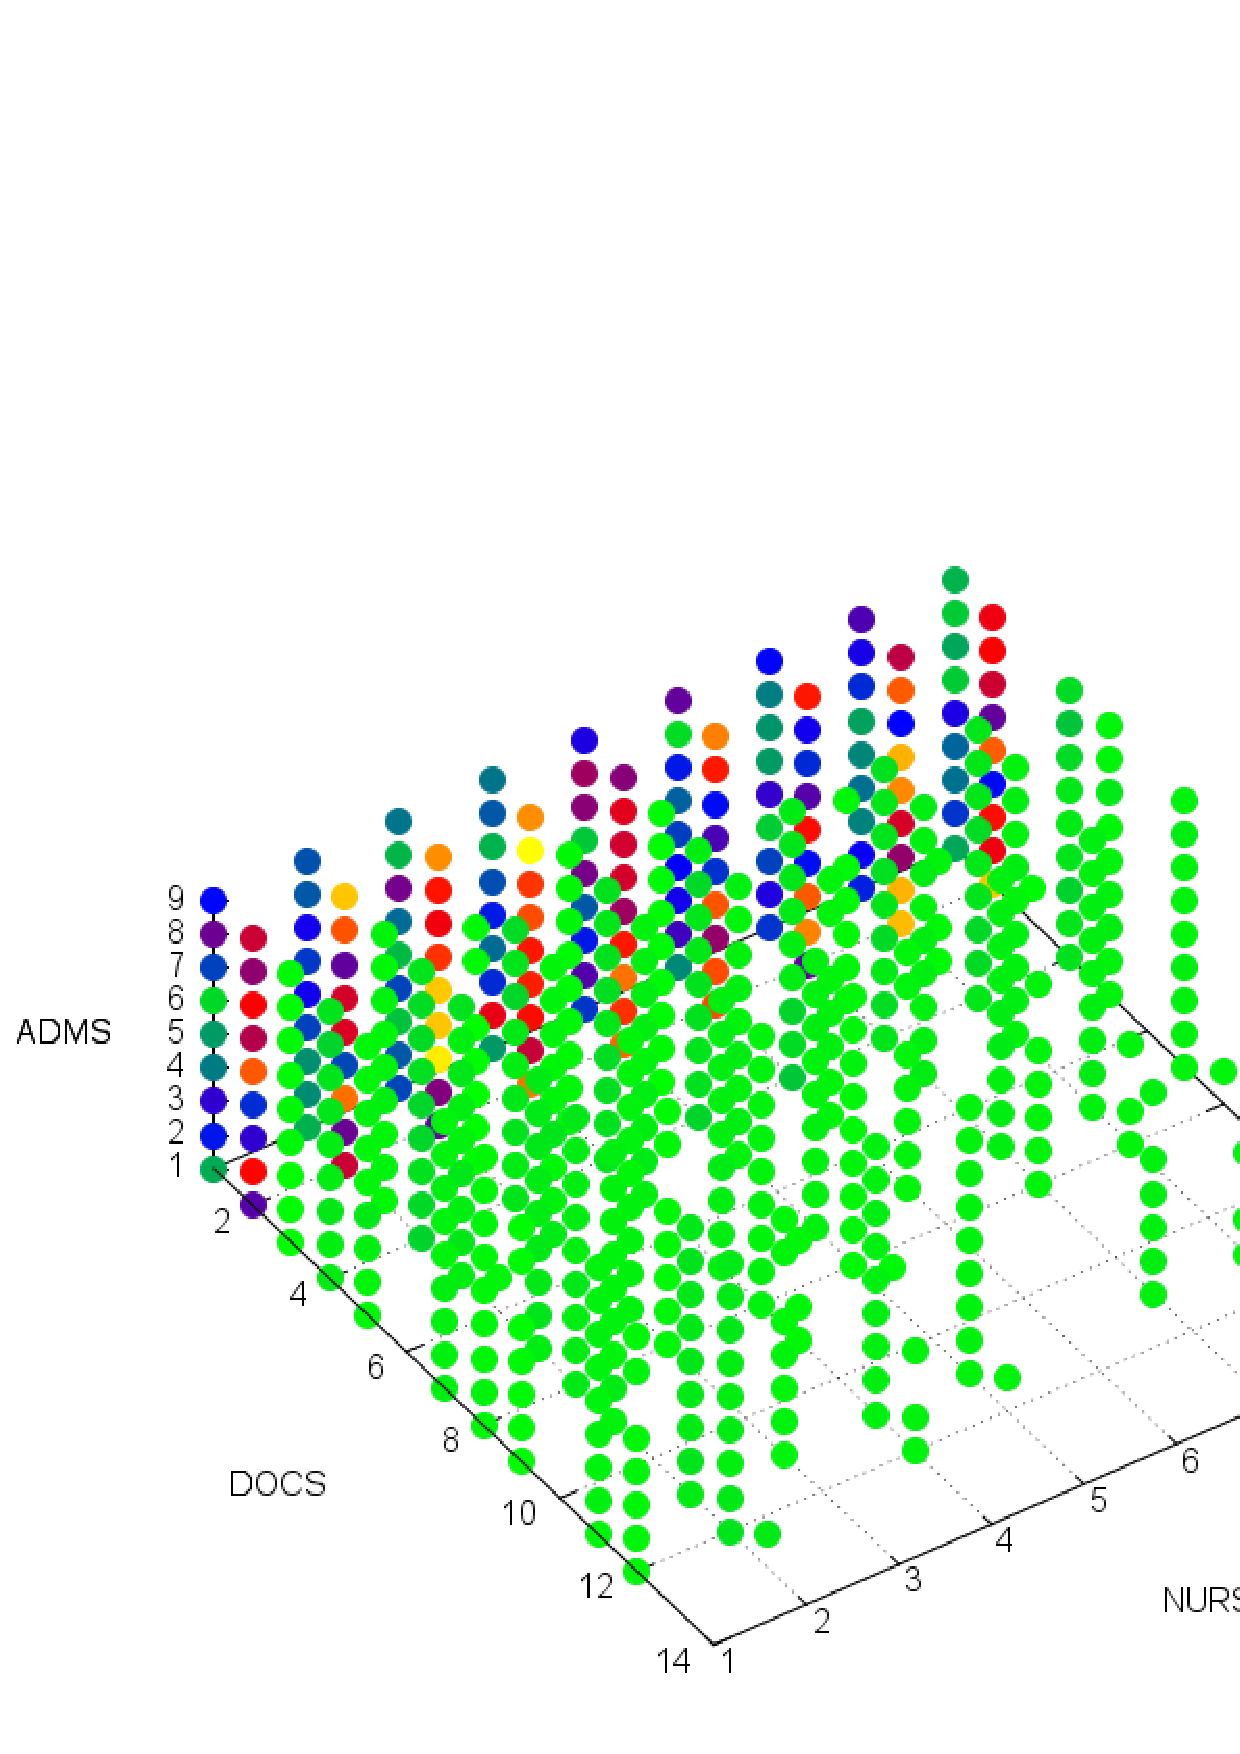
\includegraphics[width=0.88\columnwidth,height=0.2\paperheight]{figs4/3D-scatter-LoS-wo2}\caption{3D scattered graph ordered by the sort and number of staff \ref{subtab:As}
to \ref{subtab:Ds}. The green values of interest were totally scattered.
\label{fig:3D-scattered-LoS-wo}}
\end{figure}
 The second example, \ref{fig:3D-scattered-LoS-cost} shows the index
value ordered by the cost of the sanitary staff configuration. The
green points were less scattered, but blue values and others were
mixed, showing a region not totally connected. Finally, the third
example, \ref{fig:3D-scattered-LoS-tpipe}, shows the index value
ordered by the equivalent operational patient-service time \foreignlanguage{american}{(t{*})}
of each sanitary staff configuration of \ref{subtab:As-pipe} to \ref{subtab:XRs-pipe}.
This graph shows a connected and almost ``non'' scattered green
region. %
\begin{comment}
As a result of using this equivalent operational patient-service time
\foreignlanguage{american}{(t{*})} order of each staff configuration
the axes were unique and in ascending order. 
\end{comment}


\begin{figure}[h]
\noindent \begin{centering}
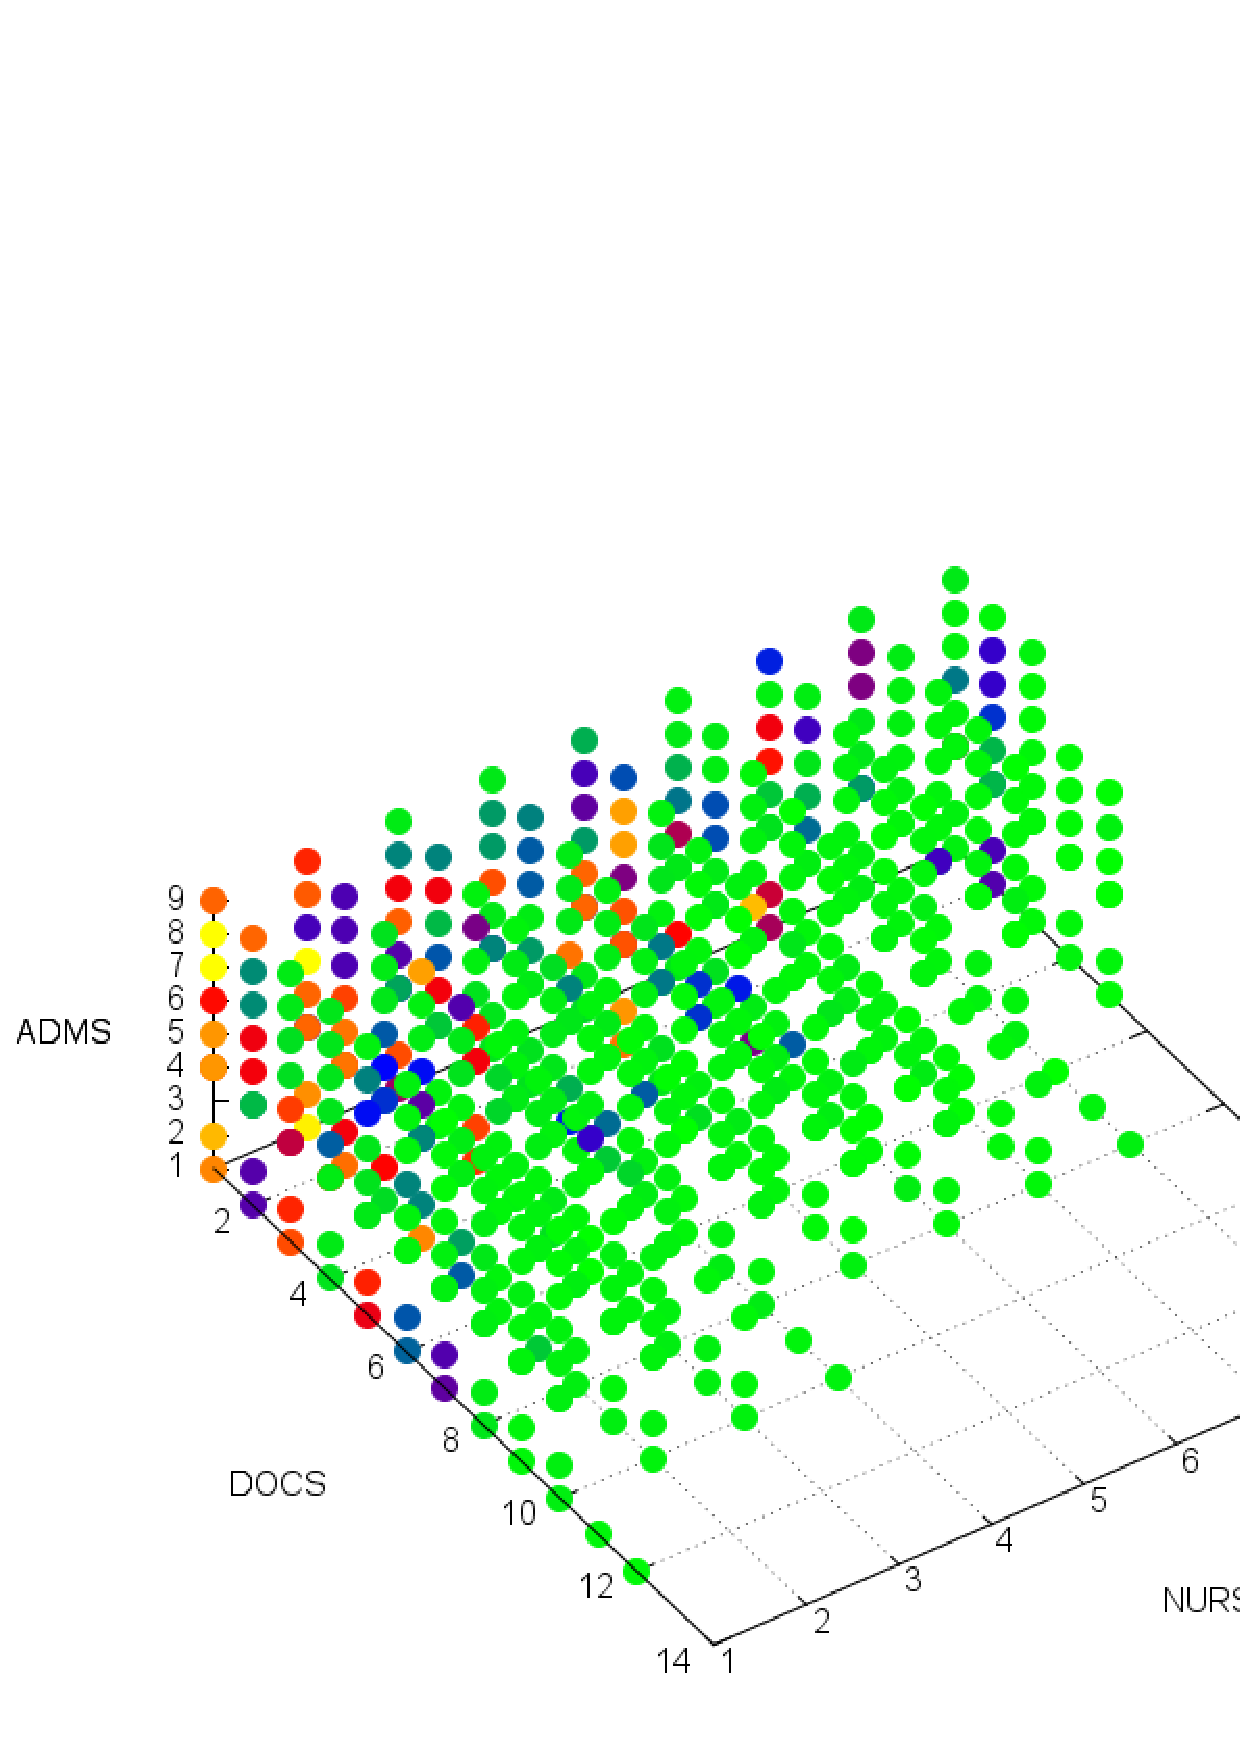
\includegraphics[width=0.88\columnwidth,height=0.2\paperheight]{figs4/3D-scatter-LoS-$2}
\par\end{centering}

\caption{3D scattered graph ordered by the cost of sanitary staff configuration.
The green values of interest were not so scattered, but not interconnected.\label{fig:3D-scattered-LoS-cost} }


\end{figure}


\section{Workloads}

In order to analyse the performance of the ED, the real average four
hundred incoming patients daily arrive to the ED of Sabadell hospital
was considered as follows. This real input was divided into four scenarios,
i.e., four different workload scenarios, up to: 4, 9, 13, and 17 incoming
patients hourly, as shown in \ref{tab:scenarios} (i.e., up to 96,
216, 312, and 408, respectively for 24hrs.).
\begin{figure}[H]
 %
\noindent \begin{centering}
\centering\foreignlanguage{british}{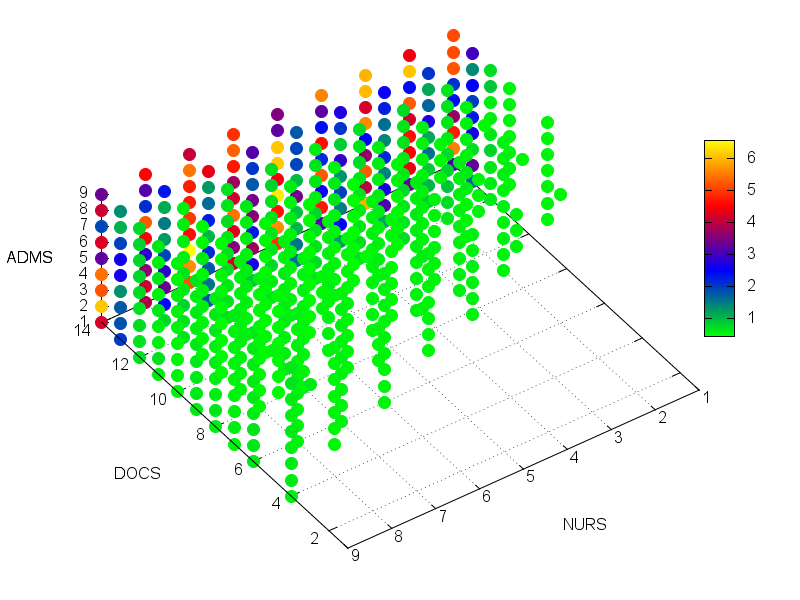
\includegraphics[width=0.88\columnwidth,height=0.2\paperheight]{figs4/3D-scatter-LoS-tpipe2}}
\par\end{centering}

  %
\caption{3D scattered graph ordered by the equivalent operational patient-service
time \foreignlanguage{american}{(t{*})} of a ``single one'' sanitary
professional of each sanitary staff configuration \ref{subtab:As-pipe}
to \ref{subtab:XRs-pipe}. The green value region of interest was
connected and almost ``non'' scattered.\label{fig:3D-scattered-LoS-tpipe} }
\end{figure}
 These different workload scenarios were used to supply different
loads to the ED, whereas the percentage of the priority level of patients
was maintained. 

\begin{table}[H]
\centering{}\caption{Incoming ED patients divided into four different workload scenarios,
up to: 4, 9, 13, and 17 patients per hour for each scenario. \label{tab:scenarios}}
\resizebox{2.3in}{!}{ %
\begin{tabular}{>{\centering}m{3.7cm}>{\centering}m{3.75cm}}
\hline 
Workload scenario number & \textbf{Incoming patients (hourly)} \tabularnewline
\hline 
1 & 4\tabularnewline
2 & 9\tabularnewline
3 & 13\tabularnewline
4 & 17\tabularnewline
\hline 
\end{tabular}}
\end{table}
\clearpage{}


\section{Evaluation Metrics}

The set of metrics used in this work were: the length of stay (LoS)
of the patients in the ED; the number of attended patients per day
(Throughput); and a compound index, the product of the cost of a given
sanitary staff configuration times patient length of stay (CLoS).

Furthermore, the computing time of each of the proposed optimisation
method is measured in order to observe the gains in reducing computing
time of the methodology proposed.\\


All simulations of the ED optimization cases analysed in this work
were carried out in a Linux cluster of the CAOS Department of the
UAB, which has 608 computing cores and 2.2TB of RAM, that is composed
of: 9 nodes of a dual-4 core Intel Xeon E5430, 2.6GHz, 16GB RAM; 1
node of 2xdual-6 core Intel Xeon E5645, 2.4GHz, 24GB RAM; and 8 nodes
of 4x16-cores AMD Opteron ``Interlagos'', 1.66GHz, 256 GB RAM, all
in a switched 1GigE network.


\section{Evaluation Method}

The evaluation of the proposed methodology was aimed to confirm the
correct operation of both the pipeline approach (PA) and the MC plus
the K-means methods, described in \ref{chap3:Math}. To this end,
we have first performed the exhaustive search (ES) to use as baseline
method. The second step of this evaluation consists on applying the
coarse grained phase, using either the PA, the MC plus K-means methods,
or both. Finally, the fine grained phase is apply in the promising
regions found in the previous step. 

In order to evaluate quantitatively the proposal methodology two case
studies were set. The first of them, namely case study A, was performed
using the agent-based ED simulator version 1.1. This case study is
further described in \ref{sub:Case-Study-A}. The second case or case
study B was performed using the agent-based ED simulator version 1.2
(the current version). This case study is further described in \ref{sub:Case-Study-B}.

In both case studies, only patients identified as triage level 4 and
5 are served at the stage of diagnosis-treatment phase, the three
metrics, and the four different workloads stated above were tested,
and the period simulated was 24 hrs., i.e., one day of functioning
of the ED, in all the experiments. Test scenarios and evaluation results
of both case studies are explained in detail in the following sections.\\


It is important to remind that the actions and interactions corresponding
to the admission and triage processes have been totally implemented,
but in the case of diagnostic and treatment phase, respecting to the
priorities of the Sabadell Hospital ED currently only the level 1
was implemented. In such level 1 only patients identified with priority
level 4 or 5 (less urgent, and non-urgent, respectively \ref{sec:active-agents})
were taken care of. Nevertheless, all incoming patients were triaged.
Once patients have been triaged, only patients identified as triage
level 4 and 5 were served at the stage of diagnosis-treatment phase.

